% ------------------------------------------------------------------------------
% TYPO3 CMS 8 LTS - What's New - Chapter "Backend User Interface" (English Version)
%
% @author	Michael Schams <schams.net>
% @license	Creative Commons BY-NC-SA 3.0
% @link		http://typo3.org/download/release-notes/whats-new/
% @language	English
% ------------------------------------------------------------------------------
% LTXE-CHAPTER-UID:		07b25346-95b1df21-a6ebe09a-49f53f41
% LTXE-CHAPTER-NAME:	Backend User Interface
% ------------------------------------------------------------------------------

\section{Backend User Interface}
\begin{frame}[fragile]
	\frametitle{Backend User Interface}

	\begin{center}\huge{\color{typo3darkgrey}\textbf{Backend User Interface}}\end{center}
	\begin{center}\large{\textit{The TYPO3 CMS administration interface got even better}}\end{center}

\end{frame}

% ------------------------------------------------------------------------------
% LTXE-SLIDE-START
% LTXE-SLIDE-UID:		fd6d762a-b268caf0-cb6f9195-f553e035
% LTXE-SLIDE-TITLE:		Set the alternative backend logo via Extension Manager
% ------------------------------------------------------------------------------
\begin{frame}[fragile]
	\frametitle{Backend User Interface}
	\framesubtitle{Alternative Logo}

	The backend logo in the upper left corner can now be configured in the extension configuration
	of EXT:backend in the Extension Manager.\newline
	Configuration options are:

	\begin{itemize}
		\item resource as a relative path of the TYPO3 installation\newline
			\smaller
				e.g. "\texttt{fileadmin/images/my-background.jpg}"
			\normalsize

		\item path to an extension\newline
			\smaller
				e.g. "\texttt{EXT:my\_theme/Resources/Public/Images/my-background.jpg}"
			\normalsize

		\item an external resource\newline
			\smaller
				e.g. "\texttt{//example.com/my-background.png}"
			\normalsize

	\end{itemize}

	\begin{figure}
		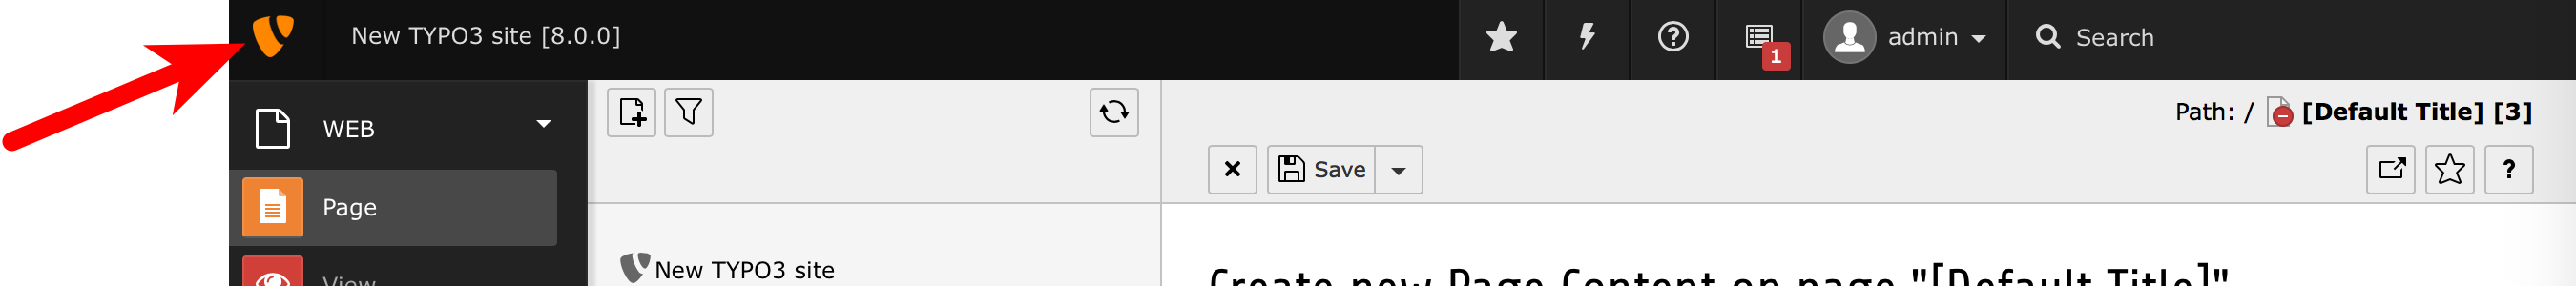
\includegraphics[width=0.7\linewidth]{BackendUserInterface/74109.png}
	\end{figure}

\end{frame}

% ------------------------------------------------------------------------------
% LTXE-SLIDE-START
% LTXE-SLIDE-UID:		75977160-b74e3317-0f697728-71b501d1
% LTXE-SLIDE-TITLE:		Mobile Responsive TYPO3 Backend
% ------------------------------------------------------------------------------

\begin{frame}[fragile]
	\frametitle{Backend User Interface}
	\framesubtitle{Mobile Responsive TYPO3 Backend}

	The TYPO3 Backend is fully mobile responsive now.

	\begin{figure}
		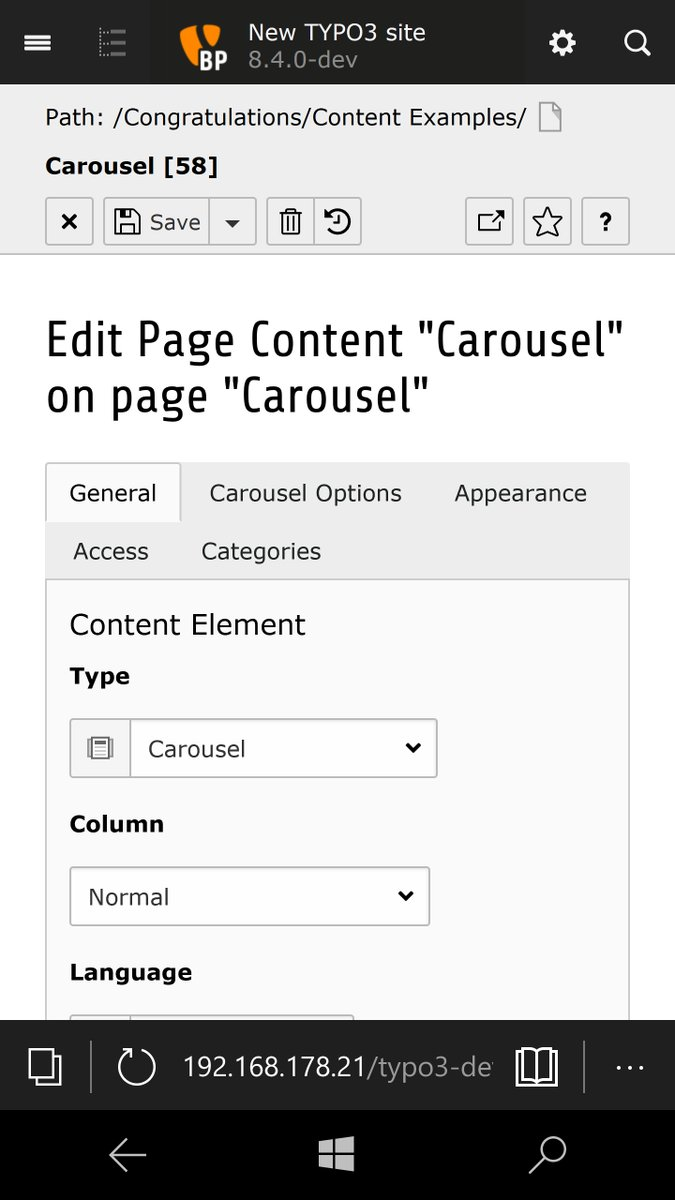
\includegraphics[width=0.25\linewidth]{BackendUserInterface/mobile-responsive-backend.jpg}
	\end{figure}

\end{frame}

% ------------------------------------------------------------------------------
% LTXE-SLIDE-START
% LTXE-SLIDE-UID:		ab5ef36b-c670fbea-fd6d762a-cb6f9195
% LTXE-SLIDE-TITLE:		Page module: drag and drop can copy elements
% ------------------------------------------------------------------------------
\begin{frame}[fragile]
	\frametitle{Backend User Interface}
	\framesubtitle{Drag \& Drop Can Copy Elements}

	Additionally to the usual drag and drop feature in the page module (that \textit{moved} content elements),
	it is now possible to create copies: press the CTRL key while dropping to create a copy of the dragged
	element. After dropping is complete, the page module will reload to make sure the new element will be
	generated with all necessary information.

	\begin{figure}
		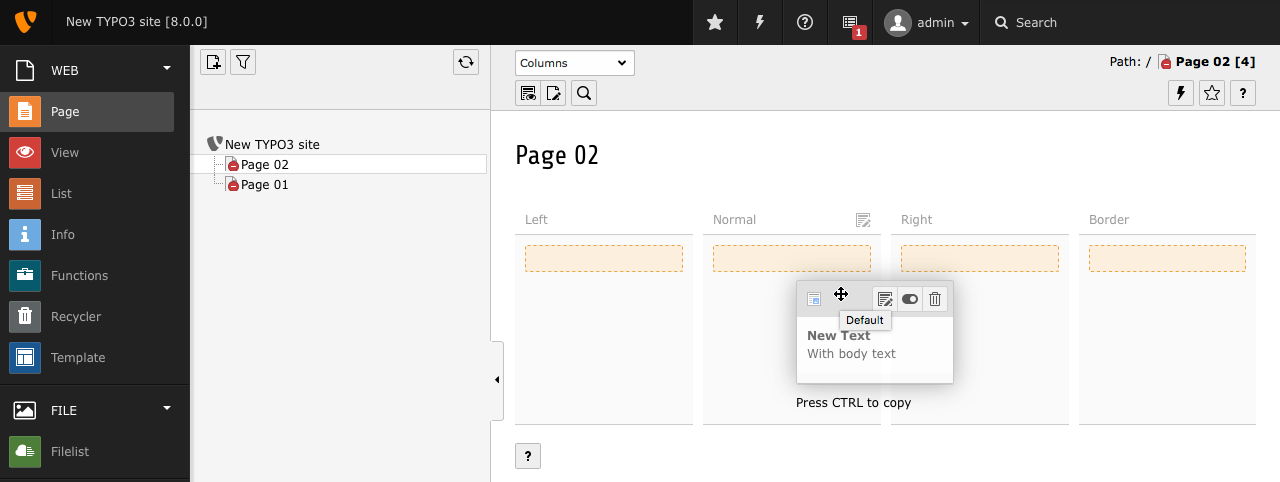
\includegraphics[width=0.7\linewidth]{BackendUserInterface/74179.png}
	\end{figure}

\end{frame}

% ------------------------------------------------------------------------------
% LTXE-SLIDE-START
% LTXE-SLIDE-UID:		14d6e262e72f00405d2bedf0096fe043
% LTXE-SLIDE-TITLE:		Feature #75880: Image Manipulation - Multiple Cropping Variants (1)
% ------------------------------------------------------------------------------
\begin{frame}[fragile]
	\frametitle{Backend User Interface}
	\framesubtitle{Image Manipulation (1)}

	\begin{itemize}

		\item Multiple aspect ratios can be configured\newline
			\small(default ratios: 16:9, 3:2, 4:3 and 1:1)\normalsize

		\item Editors can set a focal point (responsive images)\newline
			\small
				(this area of an image is still visible, even if the image is cropped,
				e.g. on small screens such as on smartphones)
			\normalsize

		\item Integrators/developers can configure \textit{crop variants} (e.g. "mobile",
			"desktop", etc.) and also use these in TCA and Fluid templates

			\begin{lstlisting}
				<f:image image="{data.image}" cropVariant="mobile" width="800">
				</f:image>
			\end{lstlisting}

			See \href{https://docs.typo3.org/typo3cms/extensions/core/8-dev/Changelog/8.6/Feature-75880-ImplementMultipleCroppingVariantsInImageManipulationTool.html}{docs.typo3.org}
			for further details.

	\end{itemize}

\end{frame}

% ------------------------------------------------------------------------------
% LTXE-SLIDE-START
% LTXE-SLIDE-UID:		23a4baef-462e7d0c-c8cd4cfc-9dac1f99
% LTXE-SLIDE-TITLE:		Feature #75880: Image Manipulation - Multiple Cropping Variants (2)
% ------------------------------------------------------------------------------
\begin{frame}[fragile]
	\frametitle{Backend User Interface}
	\framesubtitle{Image Manipulation (2)}

	\begin{figure}\vspace*{-0.6cm}
		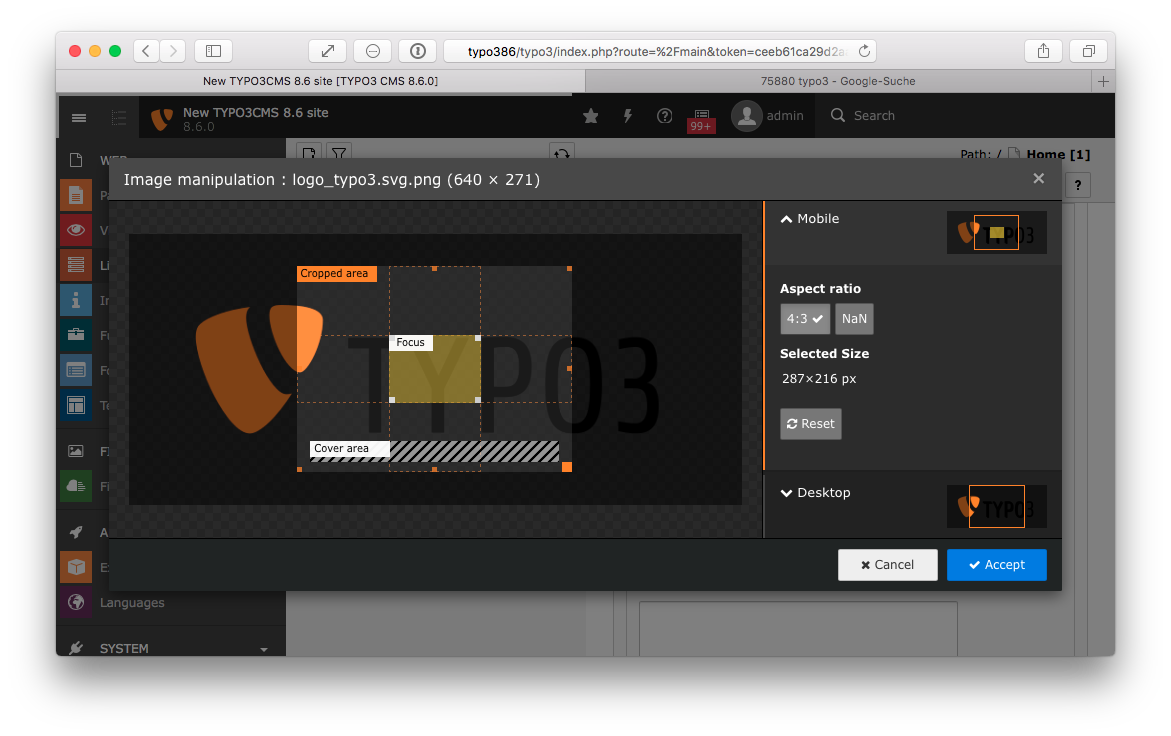
\includegraphics[width=0.90\linewidth]{BackendUserInterface/75880.png}
	\end{figure}

\end{frame}


% ------------------------------------------------------------------------------
% LTXE-SLIDE-START
% LTXE-SLIDE-UID:		7cab4dc0-cdfe9472-a3f0a874-dddf137d
% LTXE-SLIDE-TITLE:		Feature #75581: Cache clearing
% ------------------------------------------------------------------------------
\begin{frame}[fragile]
	\frametitle{Backend User Interface}
	\framesubtitle{Simplify Cache Clearing}

	The cache clearing system has been simplified by removing options in cache clear menu and
	Install Tool.

	\begin{itemize}

		\item \textbf{Flush frontend caches:}\newline
			\small
				Clears frontend and page-related caches, like before.
			\normalsize

		\item \textbf{Flush all caches:}\newline
			\small
				Clears all system-related caches, including the class loader, localization,
				extension configuration file caches and opcode caches. Rebuilding this cache
				may take some time.
			\normalsize

	\end{itemize}

	\begin{figure}
		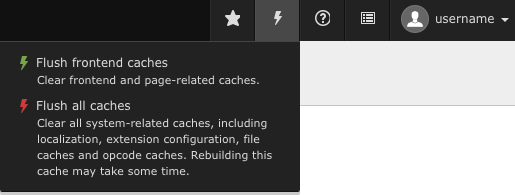
\includegraphics[width=0.45\linewidth]{BackendUserInterface/75581.png}
	\end{figure}

\end{frame}

% ------------------------------------------------------------------------------
% LTXE-SLIDE-START
% LTXE-SLIDE-UID:		a5b4032f-741b8eea-643674fb-4dc14f50
% LTXE-SLIDE-TITLE:		Feature #20446: Clear cache entry in context menu
% ------------------------------------------------------------------------------
\begin{frame}[fragile]
	\frametitle{Backend User Interface}
	\framesubtitle{"Clear Cache" Entry in Context Menu}

	A new entry has been added to the context menu of the page tree. The item is located inside "Page Actions"
	and allows to clear the cache of the selected page.

	\begin{figure}
		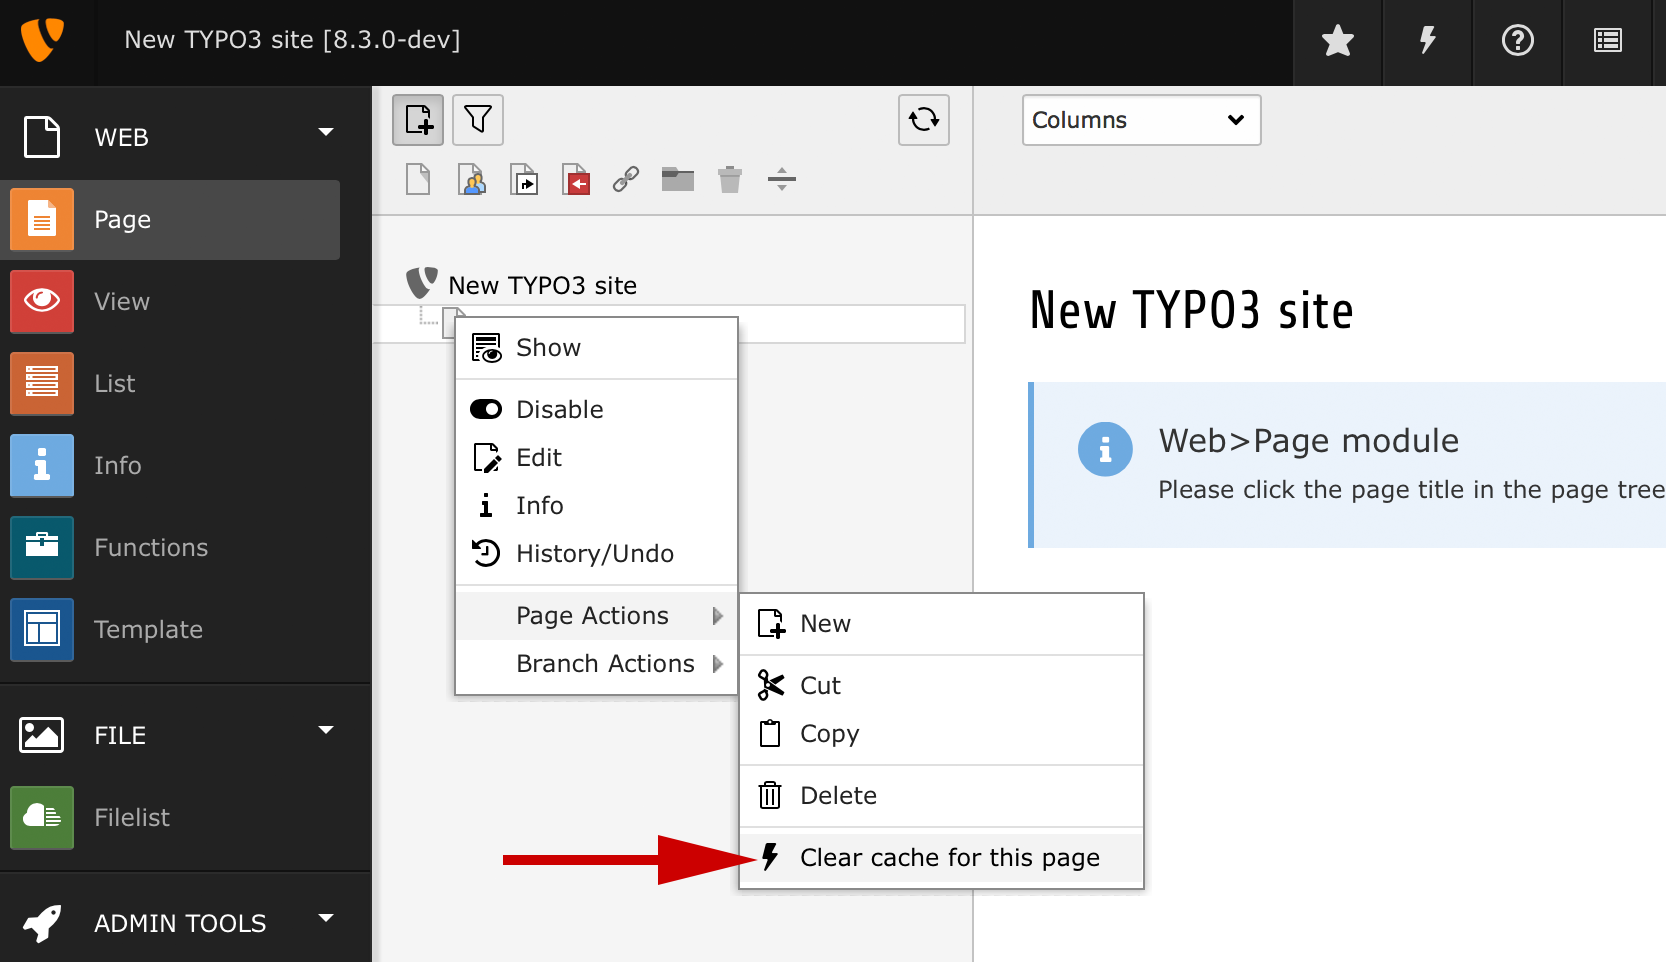
\includegraphics[width=0.70\linewidth]{BackendUserInterface/20446.png}
	\end{figure}

\end{frame}

% ------------------------------------------------------------------------------
% LTXE-SLIDE-START
% LTXE-SLIDE-UID:		e24e593c-fe9bcff9-c386db3a-79491de1
% LTXE-SLIDE-TITLE:		Workspaces (1)
% ------------------------------------------------------------------------------
\begin{frame}[fragile]
	\frametitle{Backend User Interface}
	\framesubtitle{Reworked Workspaces (1)}

	\begin{itemize}

		\item The workspace module to manage staged content has been rewritten and
			integrates much better into the visual appearance of the backend now

		\item Editors will realize straight away, it fits the overall look and feel
			due to its technical base with Twitter Bootstrap and jQuery

		\item This change also brings a performance boost and is a huge leap forward
			to a cleaner and faster TYPO3 backend with less JavaScript

	\end{itemize}

\end{frame}

% ------------------------------------------------------------------------------
% LTXE-SLIDE-START
% LTXE-SLIDE-UID:		fe9bcff9-e24e593c-79491de1-c386db3a
% LTXE-SLIDE-TITLE:		Workspaces (2)
% ------------------------------------------------------------------------------
\begin{frame}[fragile]
	\frametitle{Backend User Interface}
	\framesubtitle{Reworked Workspaces (2)}

	Screenshots of the workspace module:

	\begin{figure}
		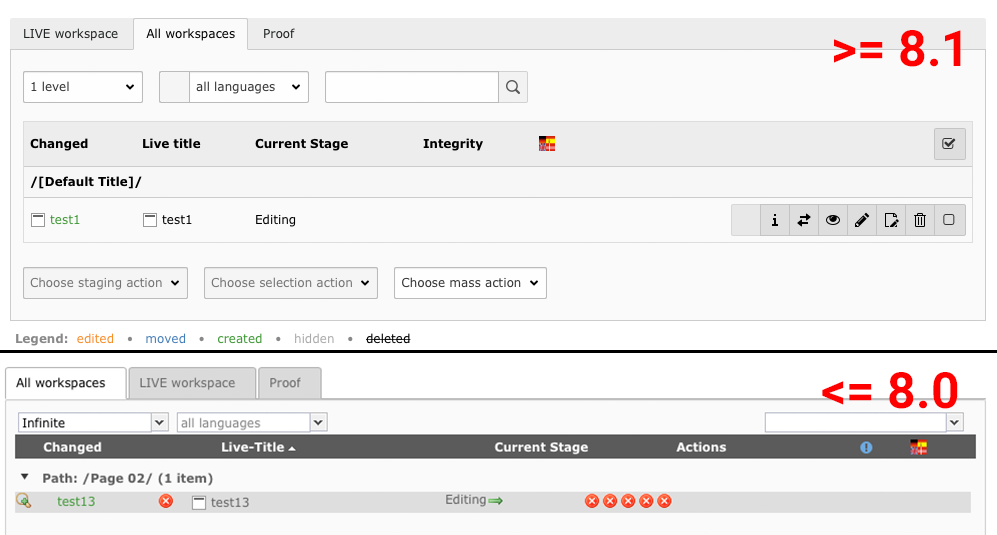
\includegraphics[width=0.85\linewidth]{BackendUserInterface/workspaces.png}
	\end{figure}

\end{frame}

% ------------------------------------------------------------------------------
% LTXE-SLIDE-START
% LTXE-SLIDE-UID:		c9dc360d-cf218f95-03f53731-03d821ad
% LTXE-SLIDE-TITLE:		#78383: Field positions in tabs streamlined (TCA)
% ------------------------------------------------------------------------------
\begin{frame}[fragile]
	\frametitle{Backend User Interface}
	\framesubtitle{Position and Order of Elements}

	\begin{itemize}
		\item The order and position of certain fields in the backend of TYPO3 has been streamlined
		\item The aim is to meet users' expectation where to find commonly used options in the user interface
		\item This is especially important for recurring field definitions and generic categories shared by a lot of records
		\item Extension authors are encouraged to follow the specified positions and orders of elements in
			the \href{https://docs.typo3.org}{official documentation}

			% TODO: update link above (waiting for Doc and Core Team to finish documentation)

	\end{itemize}

	\begin{itemize}
		\item \textit{Backend consistency is king!} :-)
	\end{itemize}

\end{frame}

% ------------------------------------------------------------------------------
